\chapter{Versuchsaufbau}
\label{cha:Versuchsaufbau}

Der verwendete Grundaufbau besteht aus dem Laserrohr, gefüllt mit einem He-Ne Gas, zwei Resonatorspiegeln, welche durch empflindliche Justierschrauben geneigt und gedreht werden können und 
einer Schiene, auf der alle Bauteile befestigt werden und parallel zur optischen Achse verschoben werden können. Das Laserrohr hat eine Länge von $l=\qty{408}{\nano\metre}$, einen Durchmesser
von $d_{HeNe} = \qty{1.1}{\milli\metre}$ und ist an Elektroden angeschlossen, sodass eine Entladung zur Anregung des Heliums stattfinden kann. Die Resonatorspiegel weisen einen Durchmesser von $d_{mirror} = \qty{12.7}{\milli\metre}$
auf. Die gekrümmten Spiegel haben jeweils einen Krümmungsradius von $r = \qty{1400}{\milli\metre}$.
Ein Bild des Grundaufbaus ist in \autoref{fig:Aufbau} zu sehen.
\begin{figure}
    \centering
    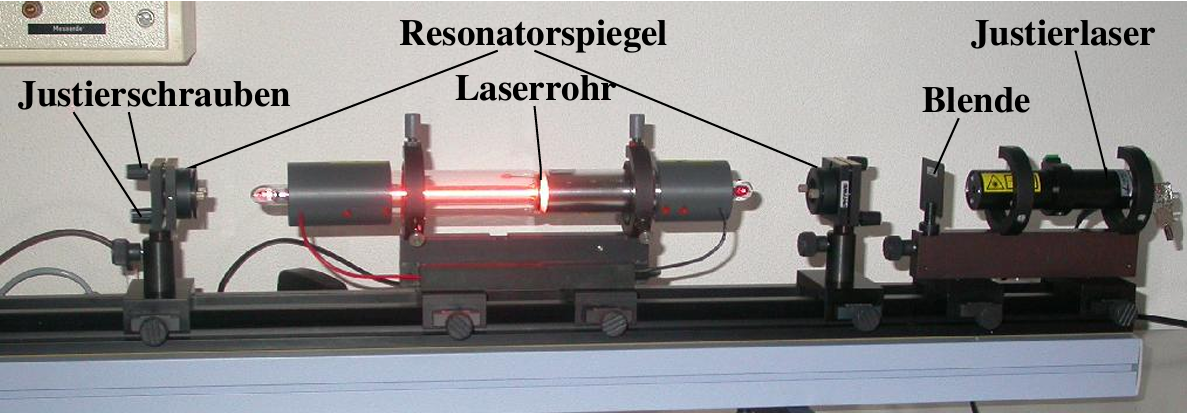
\includegraphics[width = \textwidth]{v61_bilder/Aufbau.png}
    \caption{Bild des verwendeten Grundaufbaus \cite{v61}.}
    \label{fig:Aufbau}
\end{figure}
\\An den beiden Enden des Zylinders befinden sich jeweils Brewster-Fenster, um eine einheitliche lineare Polarisation zu erzeugen und gleichzeitig geringe Verluste zu erleiden. Die Brewster Fenster
weisen eine Neigung von dem spezifischen Brewster-Winkel zur optischen Achse auf, wodurch Licht, welches parallel zur Einfallsebene polarisiert (p-polarisiert) ist, nicht abgeschwächt wird. Jener Anteil mit einer Polarisation
senkrecht zur Einfallsebene (s-polarisiert) wird leicht reflektiert. Durch den Resonator werden diese Brewster-Fenster mehrfach durchlaufen, wodurch der Anteil an p-polarisierten Licht immer höher wird.
Dadurch, dass bei der stimulierten Emission von Photonen die Polarisation des einfallenden Photons kopiert wird, entsteht am Ende einheitlich p-polarisiertes Licht mit minimalen Verlusten. Die Funktionsweise eines
Brewster-Fensters ist in \autoref{fig:Brewster} zu sehen.
\begin{figure}
    \centering
    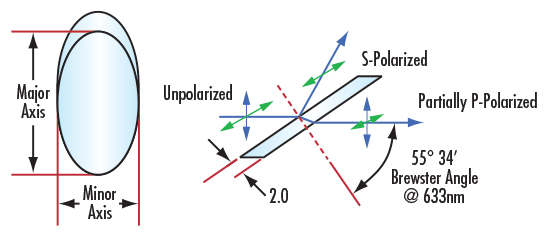
\includegraphics[width = \textwidth]{v61_bilder/Brewster.jpg}
    \caption{Schematische Darstellung der Funktionsweise eines Brewster-Fensters. Der eingezeichnete Winkel ist exemplarisch für den in diesem Versuch verwendeten Laser \cite{Brewster}.}
    \label{fig:Brewster}
\end{figure}
\\Für die Justage der Vorrichtung wird ein Justierlaser verwendet, welcher eine Wellenlänge von $\lambda = \qty{532}{\nano\metre}$ und eine Leistung von $P_{grün}= \qty{0.2}{\milli\watt}$ besitzt. Aufgrund der geringen
Leistung, kann der Laser auch während Messungen in Betrieb bleiben, er wird allerdings für ein möglichst genaues Ergebnis jedesmal abgeschaltet. Der Laser reiht sich im optischen Spektrum in einem Grünton ein,
welcher deutlich von dem roten He-Ne Laser ($\lambda = \qty{632.8}{\nano\metre}$) zu unterscheiden ist. Zu Justage werden zudem zwei Lochblenden mit kleinem Loch in der Mitte und eine Blende verwendet. Eine Loch Blende wird direkt
hinter dem Justagelaser und vor dem Spiegel positioniert und der andere hinter den zweiten Spiegel und vor die geschlossene Blende. Somit kann der Strahlengang genau nachvollzogen und justiert werden.\\
Um die Leistung des Strahls zu messen, wird in einer Versuchsreihe ein Leistungsmesser verwendet und einmal eine Photodiode. Zur Messung der Polarisation steht ein Polarisator bereit und zur Messung der Transversalmoden ein dünner Draht mit 
einem Durchmesser von $d_{Draht} = \qty{0.005}{\milli\metre}$ und eine Streulinse. Zur Messung des Frequenzspektrums wird zudem ein Spektrum Analysator gebraucht und für die Messung der Wellenlänge verschiedene Gitter.\\
Da in diesem Versuch ein Laser der Klasse 3B verwendet wird, ist besondere Vorsicht geboten und ein Ablocken des Strahlgangs beim Einbringen neuer optische Elemente nötig.

\chapter{Durchführung}
\label{cha:Durchführung}

\section{Justage der Messapparatur}
Mithilfe des Justagelasers werden zunächst alle Bauteile des Lasers (Spiegel und Laserröhre) einzeln mithilfe der Blenden justiert und schließlich zusammengebracht und 
aufeinander fein abgestimmt. Wenn der Strahl sauber justiert ist, kann der He-Ne Laser in Betrieb genommen werden. Hierfür wir ein Strom von $I=\qty{6.5}{\milli\ampere}$
angelegt, um eine Entladung des Heliums zu erzwingen. Es kann hier nötig sein, den Laser noch einmal fein zu justieren. Wenn auf einem optischen Schirm hinter dem Auskopplungsspiegel
zu erkennen ein deutlicher roter Punkt zu erkennen ist, wurde richtig justiert und die Messungen können gestartet werden. Während der einzelnen Versuchsteile kann es immer wieder nötig sein
den Aufbau nachzujustieren, um einen minimalen Leistungsverlust zu erreichen. Hier kann die Leistung mit einem Leistungsmesser immer wieder überprüft werden.

\section{Messung der Stabilitätsbedingung}
Um die Stabilitätsbedingung zu überprüfen, wird die Leistung des Laser mit einem Leistungsmesser hinter dem Auskopplungsspiegel mit zwei Konfigurationen und mehreren Resonatorlängen vermessen.
Hier werden einmal eine Konfiguration mit einem flachen und einem gekrümmten Spiegel verwendet und einmal mit zwei gekrümmten Spiegeln. Bei der Konfiguration mit zwei gekrümmten Spiegeln werden
mehr Messwerte und breitere Abstände gewählt, da die Stabilitätsbedingung hier deutlich konstanter ist.

\section{Untersuchung der Transversalmoden}
\label{sec:TEM_durch}
Um die Transversalmoden zu vermessen wird sich zu eigen gemacht, dass höheren Moden von der Intensität her immer schwächer werden. Dies bedeutet, dass die Grundmode am stärksten ist. Um die Intensität der
Grundmode ($\mathrm{TEM}_{000}$) in Abhängigkeit der Entfernung orthogonal zur Ausbreitungsrichtung des Strahls zu vermessen, wird der Strahl mit einer Streulinse gebeugt und mit einer Photodiode die Leistung vermessen. Die Leistung
wird hier für mehrere Abstände zum Mittelpunkt entnommen. Für die erste Mode ($\mathrm{TEM}_{100}$) kann ein dünner Draht in den Strahl Mittelpunkt gebracht werden, da hier das Maximum der Grundmode zu erwarten ist. Hierdurch wird die Grundmode starke geschwächt
und die erste Mode ist die nächst stärkere. Auch hier wird die Leistung wieder für verschiedene Abstände zum Mittelpunkt mit einer Photodiode gemessen. Zu beachten ist hier, dass der Draht in den Resonator mit eingebracht werden muss,
da ein Draht hinter dem Auskopplungsspiegel lediglich zu einem Interferenzmuster führen würde.

\section{Bestimmung der Polarisation}
Zur Bestimmung der Polarisation wird ein Polarisator hinter den Auskopplungsspiegel gestellt und es wird die Leistung mit einem Leistungsmesser für mehrere Polarisationswinkel vermessen.

\section{Multimoden Untersuchung}
Im Laser selben gibt es durch das vorhandene Frequenzspektrum $\Delta f$ mehrere longitudinale Moden, welche dazu führen, dass es zeitliche Abhängigkeiten der Laserintensität gibt. Bestimmte Frequenzen werden abgeschwächt und andere verstärkt.
Diese Frequenzen werden mithilfe einer Photodiode und einem Spektrum Analysator für mehrere Resonatorlängen untersucht. Hiermit kann begründet werden, warum der Laser in einem Multimoden Modus verwendet
werden kann.

\section{Bestimmung der Wellenlänge}
Um die Wellenlänge des Lasers zu bestimmen, werden jeweils ein Gitter mit $\qty{1200}{\mathrm{Lines}\per\milli\metre}$ und eins mit $\qty{600}{\mathrm{Lines}\per\milli\metre}$ verwendet. Es entsteht ein Interferenzmuster.
Anhand der Abstand von zwei Maxima kann schließlich die Wellenlänge bestimmt werden. Hierfür muss außerdem der Abstand des Gitters zum optischen Schirm bekannt sein.